\section{Wellen}

\vspace{1\baselineskip}

Die \fat{Wellenfunktion} ist gegeben durch $\xi = \xi (x,t) = f(x \pm v t)$.
Wobei "$+$" Verschiebung nach \underline{links} und "$-$" nach \underline{rechts}.

$v$ ist die \fat{Phasengeschwindigkeit}, welche die Geschwindigkeit einer Welle angibt,
mit der sich eine vorgegebene Phase bewegt.

\vspace{1\baselineskip}

Die \fat{Harmonische Wellenfunktion} ist gegeben durch
\[
  \xi(x,t) = \xi_0 \sin (k(x \pm vt)) = \xi_0 \sin (kx \pm \omega t) = \xi_0 e^{i (kx \pm \omega t)}
\]
wobei
\begin{itemize}
    \item $k$: \fat{Wellenzahl} resp. \fat{Wellenvektor} (Anzahl Wellen pro Längeneinheit) mit $[k]=\frac{1}{m}$ oder $\frac{\text{rad}}{m}$
    \item $\epsilon_0$: \fat{Amplitude} mit $[\xi_0] = m$
    \item $\lambda$: \fat{Wellenlänge} mit $[\lambda] = m$
    \item $\omega$: \fat{Frequenz} in $\frac{\text{rad}}{s}$ oder $\frac{1}{s}$
\end{itemize}
Zusammenhänge:
\begin{itemize}
    \item Frequenz: $\omega = k v$ und $2 \pi f = \omega$
    \item Wellenvektor: $k = \frac{2 \pi}{\lambda}$
    \item Periode: $T = \frac{2 \pi}{\omega} = \frac{1}{f}$
\end{itemize}

\vspace{1\baselineskip}

Die \fat{Wellengleichung} in einer Dimension lautet:
\[
  \frac{\partial^2 \xi}{\partial t^2} - v^2 \frac{\partial^2 \xi}{\partial x^2}  
\]
Wir unterscheiden zwei Arten von Wellen:
\begin{itemize}
    \item \fat{Transversale Welle}: $\xi (x,t) = A f(x-vt) \hat{z}$
    
            Auslenkung senkrecht zur Propagationsrichtung.
            
            Bsp: (elastische Seilwelle)
            $v = \pm \sqrt{\frac{S}{\mu}}$ mit $S=\frac{F}{A}=$ Zugspannung und $\mu=$ Dichte (Masse
            pro Volumenelement)

    \item \fat{Longitudale Welle}: $\xi (x,t) = A f(x-vt) \hat{x}$
    
            Auslenkung parallel zur Propagationsrichtung.

            Bsp: (Federkette oder Welle im Festkörper)
            $v= \pm \sqrt{\frac{E}{\rho}}$ mit $E= \frac{F}{A} \cdot \frac{l}{\Delta l}
            = \frac{\sigma}{\epsilon_l}$
            Elastizitätsmodul und $\rho= \frac{dm}{dV} = \frac{dm}{A \ dz} =$ Dichte
\end{itemize}

\vspace{1\baselineskip}

In einer \fat{ebenen Welle} ist die Phase an jedem Ort senkrecht zur Ausbreitungsrichtung
identisch: $\xi(x,y,z,t) = A f(kz-\omega t)$

\vspace{1\baselineskip}

\fat{Polarisation} von $\vec{A} e^{i (kz-\omega t)}$:
\begin{itemize}
    \item \fat{linear}: Welle schwingt in Ebene
    \item \fat{eliptisch}: Überlagerung von zwei linear polarisierten Wellen mit Phasenunterschied
    \item \fat{zirkulär polarisiert}: Spezialfall der eliptischen Welle mit
            Phasenunterschied $\Delta \delta = \frac{\pi}{2}$
\end{itemize}

\vspace{1\baselineskip}

\fat{Wellengleichung in 3D}: Für $\xi := \vec{\xi}(\vec{r},t) = \vec{A} e^{i (\vec{k} \cdot \vec{r} - \omega t)}$
\[
    \frac{1}{v^2} \frac{\partial^2 \xi}{\partial t^2} - \frac{\partial^2 \xi}{\partial x^2}
    \frac{\partial^2 \xi}{\partial y^2} - \frac{\partial^2 \xi}{\partial z^2} 
    = \frac{1}{v^2} \frac{\partial^2 \xi}{\partial t^2} - \Delta \xi
    = 0
\]

\pagebreak

\fat{Wellengleichung für Kugelwellen}:

Für $\xi := \vec{\xi}(\vec{r},t) = \vec{A} e^{i (\vec{k} \cdot \vec{r} - \omega t)}$
\[
    \frac{1}{v^2} \frac{\partial^2 \xi}{\partial t^2} = \klammer{\frac{\partial^2}{\partial r^2} + \frac{2}{r} \frac{\partial}{\partial r}} \xi
\]

\vspace{1\baselineskip}

\begin{minipage}{0.2\textwidth}
    \fat{kinetische \\ Energiedichte}:
    \[
        \frac{dT}{dV} = \frac{1}{2} \rho \klammer{\frac{\partial \vec{\xi}}{\partial t}}^2  
    \]
\end{minipage}
\begin{minipage}{0.2\textwidth}
    \fat{elastische \\ Energiedichte}:
    \[
          \frac{dE_{el}}{dV} = \frac{1}{2} E \klammer{\frac{\partial \vec{\xi}}{\partial x}}^2
    \]
\end{minipage}

\vspace{1\baselineskip}

\fat{Gesammtenergie}:
\[
    \frac{d W}{d V} = \frac{d E_{el}}{dV} + \frac{dT}{dV} =
    \rho v^2 \klammer{\frac{\partial f}{\partial u} \frac{\partial u}{\partial x}}^2  
\]
konkret für Welle $\xi(x,t)= A \cos (kx-\omega t)$ mit Phasengeschw. $v=\frac{\omega}{k}$
\[
    \frac{dW}{dV} =   \rho v^2 k^2 A^2 \sin^2 (kx-\omega t)
    = \rho \omega^2 A^2 \sin^2 (kx-\omega t)
\]

Wir definieren die \fat{mittlere Energiedichte} als:
\[
    \left\langle \frac{dW}{dV} \right\rangle  = \frac{1}{T} \int_0^T \frac{dW}{dV} (x,t) dt
    = \frac{1}{2} \rho \omega^2 A^2
\]

Die \fat{Energieflussdichte} (/der \fat{Poynting-Vektor}) $S$ ist diejenige Energie, welche pro
Zeit durch ein zum Fluss orthogonalen Flächenelement steht.
\[
    \vec{S} = \frac{d^2 W}{da \cdot dt} \cdot \frac{d \vec{a}}{\abs{d \vec{a}}}  
    \quad \text{ mit } \quad
    [S] = \frac{J}{m^2 s} = \frac{W}{m^2}
\]

Die \fat{Intensität} ist der Betrag von $S$: $I = \abs{S}$ und wird auch als
\fat{Energiestrom} bezeichnet. Die \fat{mittlere Intensität} ist:
\[
    \left\langle I \right\rangle = \frac{1}{2} \rho \omega^2 A^2 v
    = \frac{1}{2} \rho \frac{\omega^3}{k} A^2  
    = \frac{P}{A} = \frac{\text{Leistung}}{\text{Oberfläche}}
\]
Mittlerer Energiestrom der durch die gesammte Kugeloberfläche im Abstand $r$
hindurchtretenden Welle:
\[
    \dot{W} = \frac{1}{2} \rho \omega^2 \klammer{\frac{A_0}{r}}^2 \cdot v \cdot 4 \pi r^2  
\]

\vspace{1\baselineskip}

\fat{Superpositionsprinzip}: Summe zweier Wellen ist wieder eine Welle.
Hilfreiche Trigonometrische Additionstheoreme:
\begin{align*}
    \sin(x \pm y) &= \sin (x) \cdot \cos (y) \pm \cos(x) \cdot \sin(y)
    \\
    \cos(x \pm y) &= \cos(x) \cdot \cos(y) \mp \sin(x) \cdot \sin(y)
    \\
    \sin(x) + \sin(y) &= 2 \cdot \sin \klammer{\frac{x+y}{2}} \cdot \cos \klammer{\frac{x-y}{2}}
    \\
    \cos(x) + \cos(y) &= 2 \cdot \cos \klammer{\frac{x+y}{2}} \cdot \cos \klammer{\frac{x-y}{2}}
    \\
    \cos(x) - \cos(y) &= -2 \cdot \sin \klammer{\frac{x+y}{2}} \cdot \sin \klammer{\frac{x-y}{2}}
    \\
    \sin(x) \cdot \sin(y) &= \frac{1}{2} \klammer{\cos(x-y)-\cos(x+y)}
    \\
    \cos(x) \cdot \cos(y) &= \frac{1}{2} \klammer{\cos(x-y)+\cos(x+y)}
    \\
    \sin(x) \cdot \cos(x) &= \frac{1}{2} \klammer{\sin(x-y) + \sin(x+y)}
\end{align*}
Für zwei Wellenfunktionen $\xi_1 , \xi_2$ heisst das:
\begin{align*}
    \xi(x,t) &= \xi_1(x,t) + \xi_2 (x,t) = A \sin (kx_1 - \omega t) + A \sin (kx_2 - \omega t + \delta) \\
    &= 2 A \cos \klammer{\frac{\delta + k \Delta x}{2}} \sin \klammer{kx_1 - \omega t + \frac{\delta + k \Delta x}{2}}
\end{align*}

\pagebreak

Dabei beschreibt der Kosinus-Term die Amplitude und der Sinus-Term eine harmonische Welle.
Es gibt zwei Arten:
\begin{itemize}
    \item \fat{konstruktive Interferenz}:    
        neue Phase ganzzahliges Vielfaches von $\pi$: $\frac{1}{2} (\delta + k \Delta x) = n x$
    \item \fat{destruktive Interferenz}:    
        neue Phase halbzahliges Vielfaches von $\pi$: $\frac{1}{2} (\delta + k \Delta x) =
        \klammer{n+\frac{1}{2}} \pi$
\end{itemize}

\vspace{1\baselineskip}

\fat{Reflexion und Transmission}
\begin{itemize}
    \item \fat{einlaufende Welle}: $\xi_A (x,t) = A e^{i (k_1 x - \omega t)}$
    \item \fat{reflektierte Welle}: $\xi_R (x,t) = R e^{i(-k_1 x - \omega t + \delta_R)}$
    \item \fat{transmittierte Welle}: $\xi_T (x,t) = T e^{i (k_2 x - \omega t + \delta_T)}$
\end{itemize}
\begin{align*}
    R = \pm \frac{1 - \alpha}{1+ \alpha} A
    \quad \text{ , } \quad
    T= \frac{2A}{1+\alpha}
    \quad \text{ mit } \quad
    \alpha = \frac{k_2}{k_1} = \sqrt{\frac{S_1 \rho_2}{S_2 \rho_1}}
\end{align*}
\begin{itemize}
    \item $\alpha=1$: vollständige Transmission, $R=0$ und $T=A$.
    \item $\alpha > 1$: $R > 0$, hartes Medium, vollständige reflexion \underline{mit} einem
            \fat{Phasensprung $\pi$} $\Rightarrow R=\frac{\alpha - 1}{\alpha + 1} A$ und
            $T = \frac{2A}{1 + \alpha}$
    \item $\alpha<1$: $R > 0$, Grenzfall $\alpha = 0$: loses Seil,vollständige reflexion
            \underline{ohne} Phasensprung $\Rightarrow R = \frac{1-\alpha}{1+\alpha} A$ und
            $T = \frac{2A}{1+ \alpha}$
\end{itemize}

\vspace{1\baselineskip}

\fat{Stehende Welle}:

\vspace{1\baselineskip}

\small
\begin{tabular}{l|l|l}
    \hline \hline & fest eingespannt & einseitig eingespannt \\
    \hline Anfangsbed. & $u(x=0)=u(x=L)=0$ & $u(x=0)=0$, $u(x=L)$ \\
    & & $B=u_{0}$ \\
    & $\rightarrow A=0, k l=n \pi$ & $\rightarrow A=0, k l=\frac{2 n+1}{2} \pi$ \\
    Wellenzahl & $k_{n}=\frac{n \pi}{1}$ & $k_{n}=\frac{2 n+1}{2} \pi$ \\
    Wellenlänge & $\lambda_{n}=\frac{2 l}{n}$ & $\lambda_{n}=\frac{4 l}{2 n+1}$ \\
    Eigenfunktion & $u_{n}(x)=B_{n} \sin \left(\frac{n \pi}{\tau} x\right)$ & $u_{n}(x)=B_{n} \sin \left(\frac{2 n+1}{2} \tau x\right)$ \\
    Eigenfrequenz & $\omega_{n}=\frac{n \pi}{2} \sqrt{\frac{S}{\rho}}$ & $\omega_{n}=\frac{2 n+1}{2} \pi \sqrt{\frac{S}{\rho}}$ \\
    Grundfrequenz & $\omega_{1}=\tau \sqrt{\frac{S}{\rho}}$ & $\omega_{0}=\frac{\pi}{2} \sqrt{\frac{S}{\rho}}$ \\
    Harmonische \\ Oberwellen & $\omega_{n}=n \omega_{1}$ & $\omega_{n}=(2 n+1) \omega_{0}$ \\
    \hline \hline
\end{tabular}
\normalsize

\vspace{1\baselineskip}

Superposition von
\begin{align*}
    &\xi_1 (x,t) = A \cos(kx-\omega t) \text{ und } \xi_2 (x,t) = A \cos (-kx - \omega t + \delta_R)
    \\ &\text{ergibt:} \quad 
    \xi(x,t) = 2 A \cos \klammer{k x - \frac{\delta_R}{2}} \cos \klammer{\omega t - \frac{\delta_R}{2}}
\end{align*}
\begin{itemize}
    \item \fat{Reflexion am harten Medium}: ($\alpha >> 1$, $\delta_R = \pi$)
        \begin{align*}
            \xi(x,t) = 2A \sin(kz) \sin(\omega t)
        \end{align*}
    \item \fat{reflexion am weichen Medium}: ($\alpha < 1$, $\delta_R = 0$)
        \begin{align*}
            \xi(x,t) = 2 A \cos (kx) \cos (\omega t)
        \end{align*}
\end{itemize}

\vspace{1\baselineskip}

\fat{Prinzip von Huygens}:
Jeder Punkt einer Wellenfront kann als Ausgangspunkt einer neuen Welle, der sogenannten
Elementarwelle, betrachtet werden.
\begin{center}
    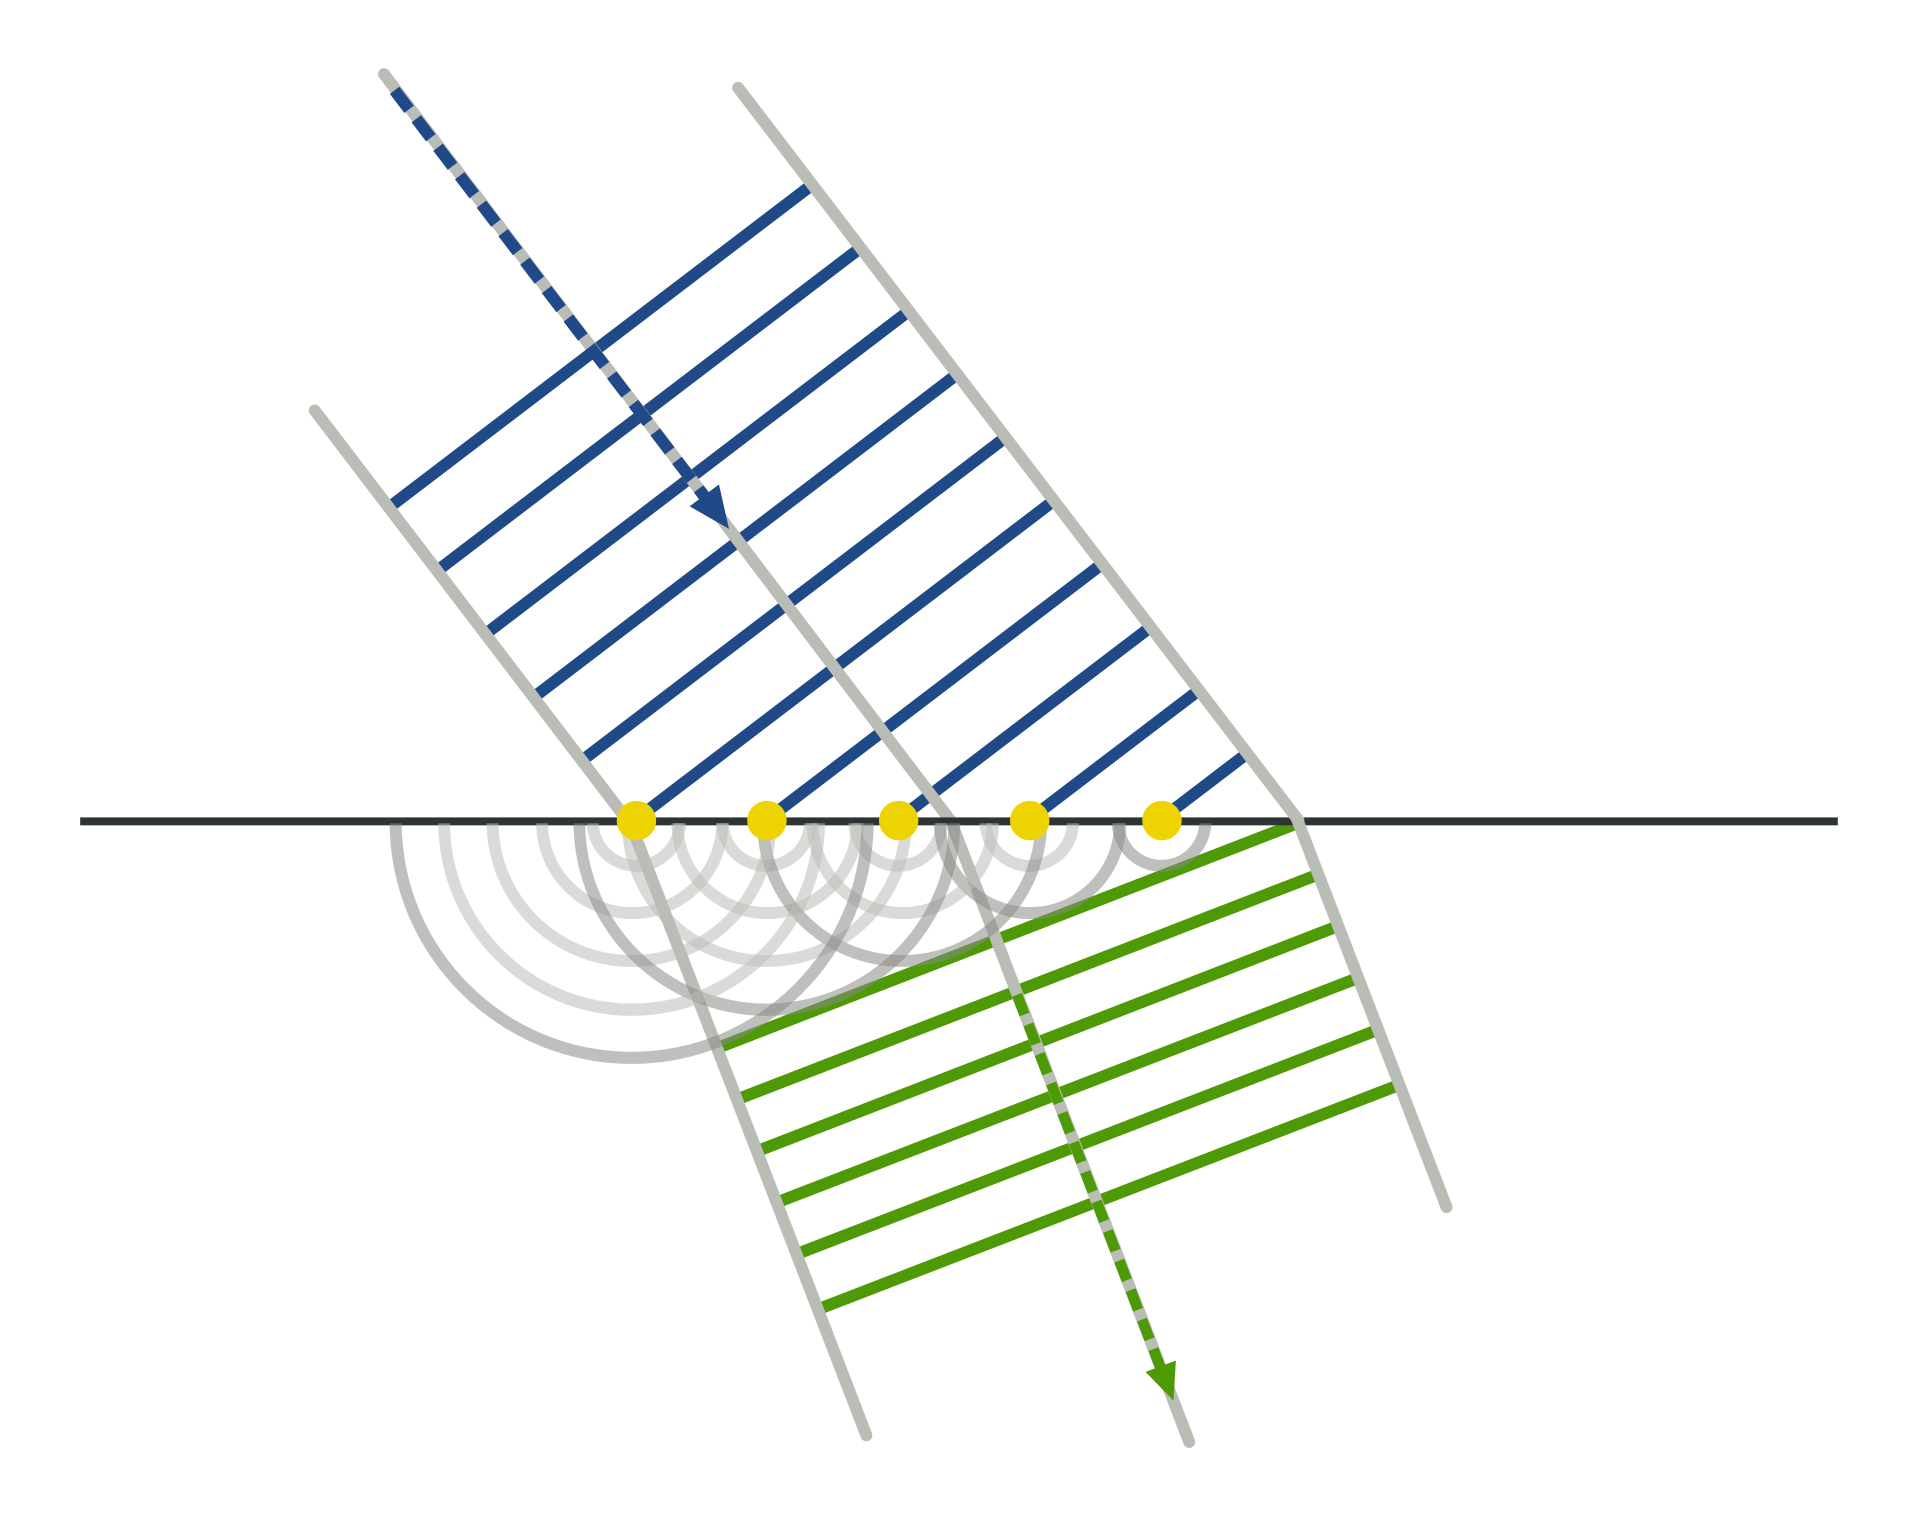
\includegraphics[width = 0.2\textwidth]{Figures/Huygen.png}
\end{center}

\pagebreak

\fat{Orte der Maximalen Verstärkung}:
$\Delta \varphi = n 2 \pi \stackrel{!}{=} k \delta \sin(\alpha)$ mit $\delta$ den Abständen
zwischen den Löchern.

\vspace{1\baselineskip}

\fat{Nullstellen der Intensität}:
Nullstellen: $\frac{k \cdot d}{2} \sin(\alpha) \stackrel{!}{=} n \cdot \pi$

Orte NST: $\sin(\alpha_{NST}) = n \frac{\lambda}{d}$
mit $d=$ Gesammtlänge der Wand, $\alpha=$ Einfallswinkel der Wellenfront.

\vspace{1\baselineskip}

\fat{Beugung} ist die Abweichung vom gradlinigen Strahlenverlauf an Grenzflächen oder
Öffnungen. Sie ist dann wichtig, wenn die Grösse der Öffnung etwa von der Grössenordnung
der Wellenlänge ist.
\begin{center}
    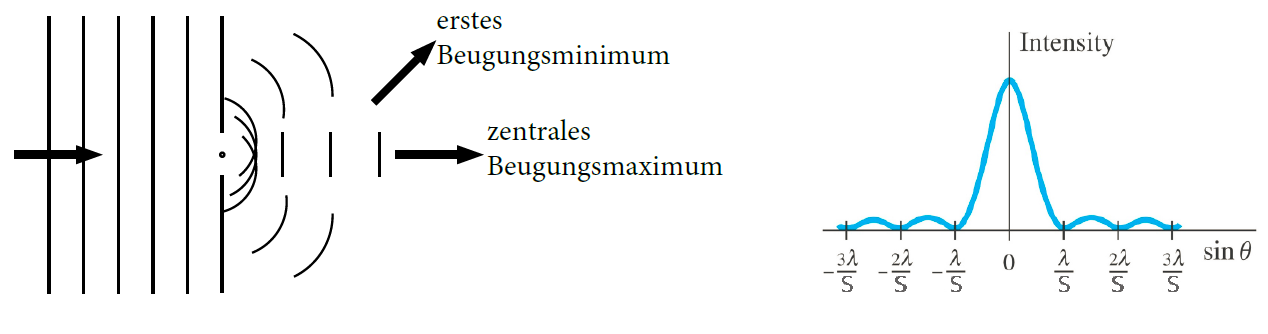
\includegraphics[width=0.4\textwidth]{Figures/Beugung2.png}
    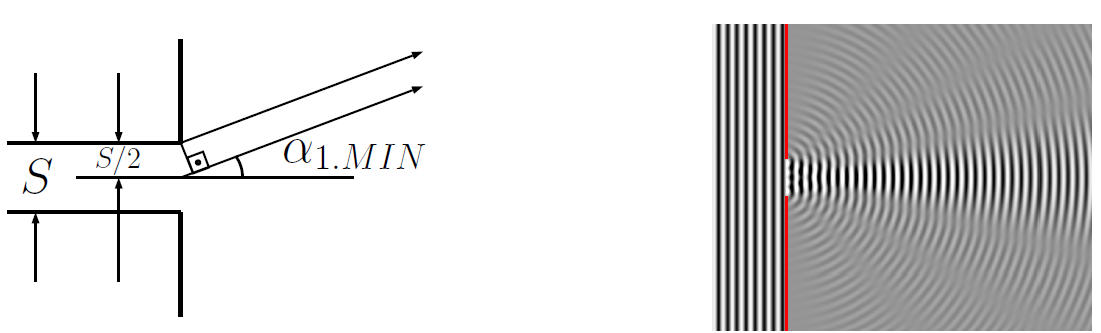
\includegraphics[width=0.3\textwidth]{Figures/Beugung3.png}
\end{center}
Für destruktive Interferenz am ersten Beugungsminimum gilt:
$\frac{S}{2} \sin (\alpha_{1,\min}) = \frac{\lambda}{2} \longrightarrow
\sin (\alpha_{1,\min}) = \frac{\lambda}{S}$

\vspace{1\baselineskip}

\fat{Der Reflexionsgesetz}
Einfallender Lichtstrahl, reflektierter Lichtstrahl und Einfallslot (Oberflächennormale
im Auftreffpunkt) liegen in einer Ebene. Einfallswinkel $\alpha_1$ und Reflexionswinkel
$\alpha_2$ - beide zum Einfallslot hin gemessen - sind gleich.

\vspace{1\baselineskip}

\fat{Das Brechungsgesetz / Snellius'sches Brechungsgesetz}
\begin{align*}
    \frac{\sin(\alpha_1)}{\sin(\alpha_2)} = \frac{c_1}{c_2} =
    \frac{c_{\text{Vakuum}}}{n_1} \frac{n_2}{v_{\text{Vakuum}}}
    = \frac{n_2}{n_1}
    = \frac{v_1}{v_2}
    = \frac{\lambda_1}{\lambda_2}
\end{align*}
mit $n=$ Brechungsindex.

\vspace{1\baselineskip}

\fat{Akustische Linsen}:
Schallgeschw. in einem Gas: $v = \sqrt{\kappa \frac{R T}{M}}$ dabei sind
$\kappa = \frac{C_p}{C_V}$, $R$ die allgemeine Gaskonstante und $M$ die Molekularmasse
des Gases.

\vspace{1\baselineskip}

\fat{Dopplereffekt}
\begin{itemize}
    \item Ruhende Quelle, bewegter Beobachter:
        \begin{itemize}
            \item Beobachter rennt von Quelle weg
                \begin{align*}
                    \nu_B = \nu_Q \klammer{1-\frac{v_B}{\lambda_{\text{emit}} \nu_Q}}
                \end{align*}
            \item Beobachter rennt auf Quelle zu
                \begin{align*}
                    \nu_B = \nu_Q \klammer{1+\frac{v_B}{\lambda_{\text{emit}} \nu_Q}}
                \end{align*}
        \end{itemize}
    \item Ruhender Beobachter, bewegte Quelle:
        \begin{itemize}
            \item Quelle entfernt sich vom Beobachter
                \begin{align*}
                    \nu'_B = \nu'_Q \klammer{1-\frac{v_Q}{\lambda_{\text{emit}} \nu_Q}}^{-1}
                \end{align*}
            \item Quelle bewegt sich auf den Beobachter zu
                \begin{align*}
                    \nu'_B = \nu'_Q  \klammer{1+\frac{v_Q}{\lambda_{\text{emit}} \nu_Q}}^{-1}
                \end{align*}
        \end{itemize}
\end{itemize}

\vspace{1\baselineskip}

\fat{Schockwelle}
Eine Schockwelle breitet sich im \fat{Mach'schen} Kegel aus. Es gilt:
$\vartheta = \arcsin \klammer{\frac{\lambda \nu}{v_Q}}$
Das Verhältnis $\frac{v_Q}{\lambda \nu}$ wird als \fat{Mach'sche Zahl}
bezeichnet.